\section{Evaluation}
\label{sec:evaluation}
Here we evaluate how our algorithm satisfies the properties we set up as the goodness-of-split criteria.

\subsection{Visually Rich}

A visualization of a data relationship appears useful when it has a visually salient pattern that translates to some simple model of the relationship, for example, a linear trend. Visual pattern measures, such as scagnostics that non-parametrically characterize the distributional shape seen in a scatterplot, can distill structure missed by ANOVA based analysis. For example, consider the bivariate relationship between linolenic and linoleic in Figure~\ref{fig:vrich_all} from the olive oils dataset~\cite{Forina1983}, which represents eight chemical measurements on different specimens of olive oil produced in various regions in Italy. There appears to be visually striking clumps and striation patterns overlaid. An analyst might wonder whether these patterns can be isolated and explained by any of the other dimensions in the dataset.
 
\begin{figure}
 \centering 
	 \begin{subfigure}{1.25in}
		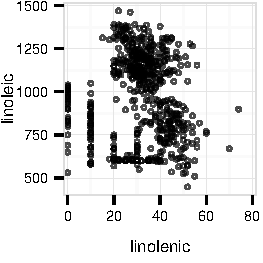
\includegraphics[width=1.25in]{images/linolenic-linoleic.pdf}
		  \caption{}
		 \label{fig:vrich_all}
	\end{subfigure}
	 \begin{subfigure}{2.5in}
		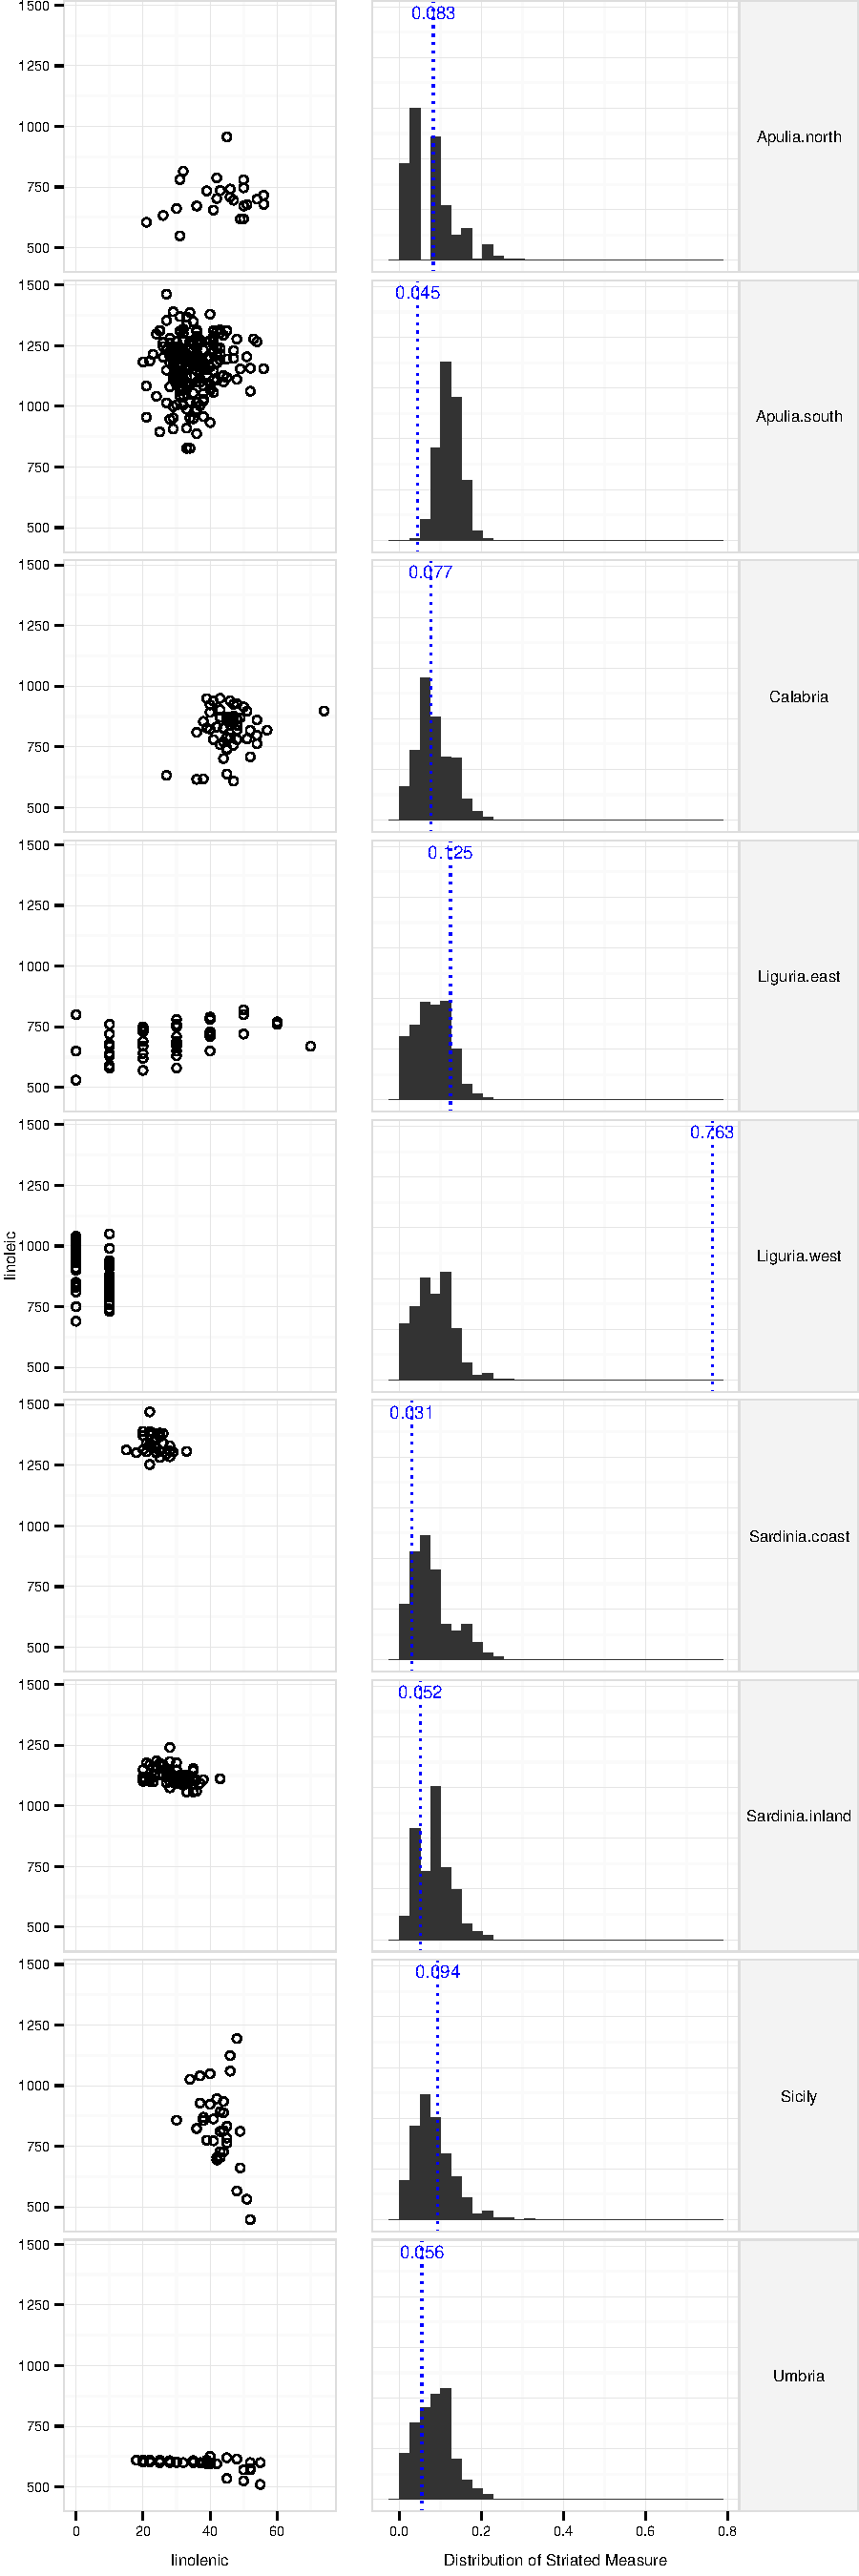
\includegraphics[width=2.5in]{images/15_2321946775352-region.pdf}
		  \caption{}
		 \label{fig:vrich_sm}
	\end{subfigure}
	  \caption{(a) User-selected bivariate relationship of two chemicals in the Olive oils dataset. (b) The highest ranked small multiple on the Striation scagnostic pulls apart the striated patterns from the original bivariate relationship. }
\end{figure}

Using the Striation scagnostic, our approach ranks the "Region" variable as the best partitioning dimension for isolating such patterns. Figure~\ref{fig:vrich_sm} reveals the clean isolation of the striation pattern for olive oils from the Liguria region and the distinctive measurement structures of linoleic values for the Umbria region. This small multiple explains the visually rich patterns seen in Figure~\ref{fig:vrich_all}.

\subsection{Informative}

When a small multiple display reveals unexpected or different structure than that seen in the original view, it adds to the user's understanding of the dataset. Different visual patterns function as an indicator of the partitioner variable's explanatory power and its independence relative to the response variables being examined.

\begin{figure}
 \centering 
	 \begin{subfigure}{1.25in}
		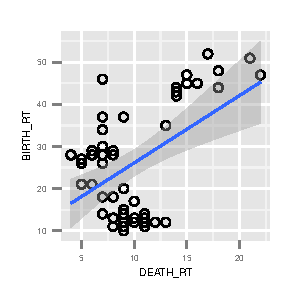
\includegraphics[width=1.25in]{images/DEATH_RT-BIRTH_RT.pdf}
		  \caption{}
		 \label{fig:informative_all}
	\end{subfigure}
	\begin{subfigure}{3in}
		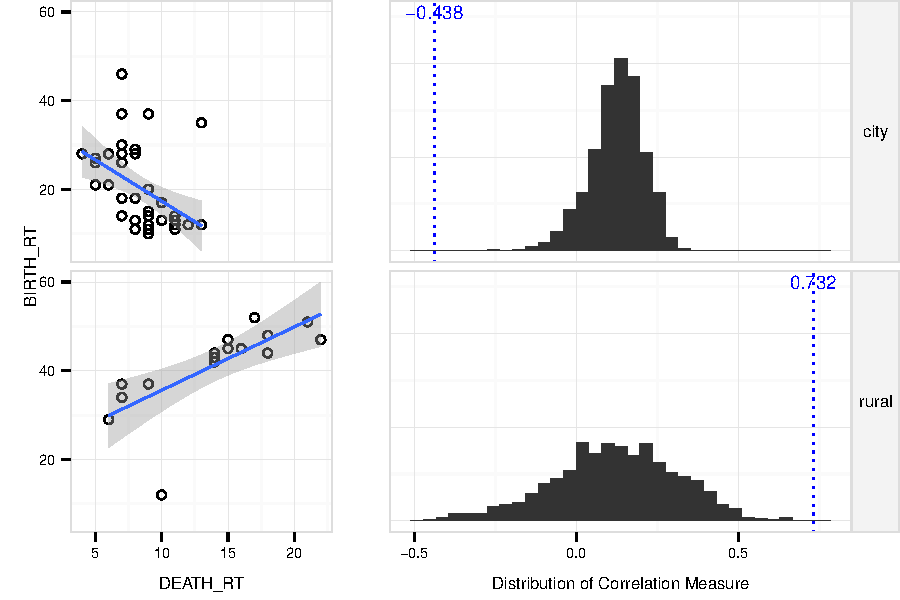
\includegraphics[width=3in]{images/6_84034106410344-URBAN.pdf}
		 \label{fig:informative_sm}
		  \caption{}
	 \end{subfigure}
	\begin{subfigure}{3in}
		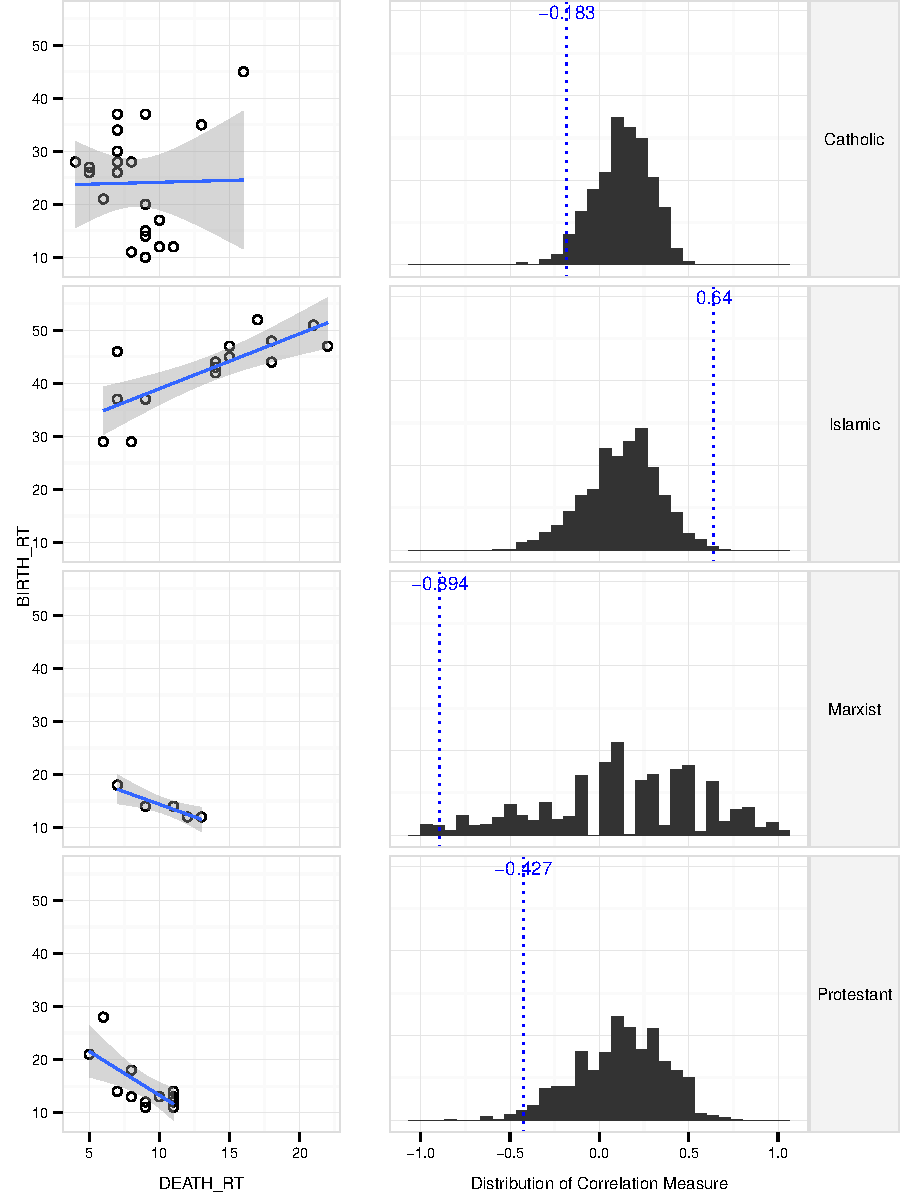
\includegraphics[width=3in]{images/2_48595929670884-LEADER.pdf}
		  \caption{}
		 \label{fig:informative_sm_big}
	 \end{subfigure}
	  \caption{(a) User-selected relationship between birth and death rates for countries around the world. (b) The highest ranked small multiple display shows partitions that reveal strong opposite trends that was not seen in the original view. (c) The lowest ranked small multiple display that reveals interesting correlations but is not parsimonious.}
\end{figure}
An illustration of an informative view involves the use of the Monotonic scagnostic  which is the ranked Spearman correlation coefficient and the Ourworld dataset of UN statistics on world countries~\cite{Wilkinson2005GG,Wilkinson2008}. We want to determine how to partition the bivariate relationship between Birth rate and Death rate seen in Figure~\ref{fig:informative_all}. The highest ranked small multiple is that determined by the variable Urban that partitions the data into two categories - city with $40$ points and rural with $17$ points. This variable can be considered a confounding covariate, the unexamined field that has an effect on the data pattern. Figure~\ref{fig:informative_sm} shows that the Birth rate is negatively correlated with Death rate in cities and positively correlated in rural settings. The negative correlation is contrary to the pattern in the original view. As such it is an example of Simpson's paradox when aggregate numbers are affected by changes in the relative size and value of the subpopulations. 
 
Figure~\ref{fig:informative_sm_big} is another informative small multiple display determined by the religion of the Leader of the countries. However, this variable has more partitions and weaker patterns as each has lower support. 

\subsection{Support}

\begin{figure}
\centering
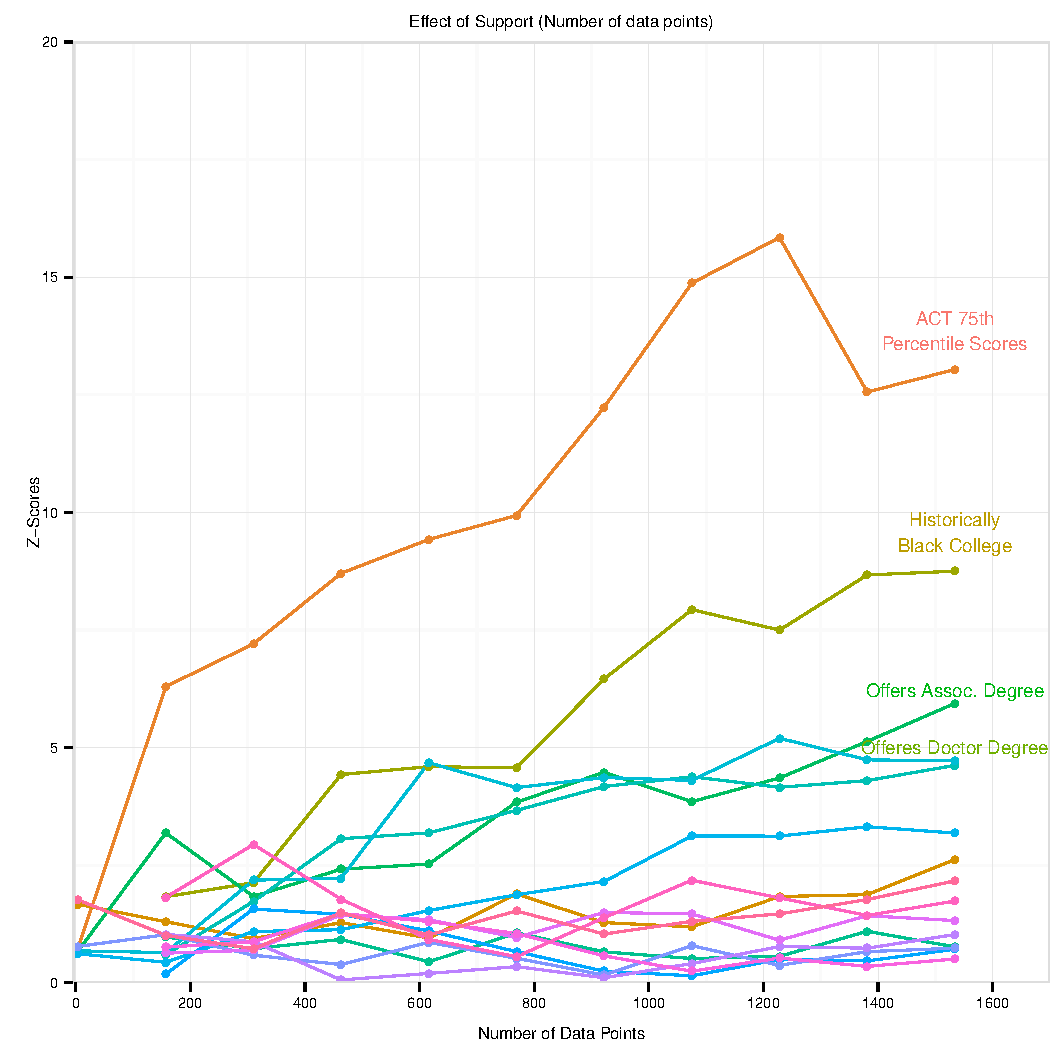
\includegraphics[width=3.25in,height=3.25in]{images/support.pdf}
  \caption{The effect of support on the combined z-scores ranking of partitioning dimensions for the data about American universities. As the number of points in the dataset decrease, the importance of the variable determined by the z-scores decrease too. }
 \label{fig:support}
\end{figure}
To examine how conservative our approach is in its assessment of interesting patterns for those partitions with low support, we conduct an experiment using the dataset about US universities. We compute the rankings based on the combined z-scores for all the partitioning dimensions in the dataset. Then we progressively remove $10\%$ of the data points at random until we barely have any points left in the dataset. At each step we recompute the rankings of the partitioning dimensions. We expect to the see the z-scores generally decreasing as the partitions have fewer points. Figure~\ref{fig:support} confirms the effect of decreasing support to the decreasing importance given to visual patterns by our approach.

\subsection{Parsimonious}
  \begin{figure}
    \centering
    \begin{minipage}[b]{1.5in}
       \begin{subfigure}[b]{\linewidth}
  	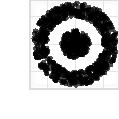
\includegraphics[width=0.65in]{images/donut1-donut2.pdf}
      \caption{}
      \label{fig:pars1}
      \end{subfigure}\\[\baselineskip]
      \begin{subfigure}[b]{\linewidth}
  	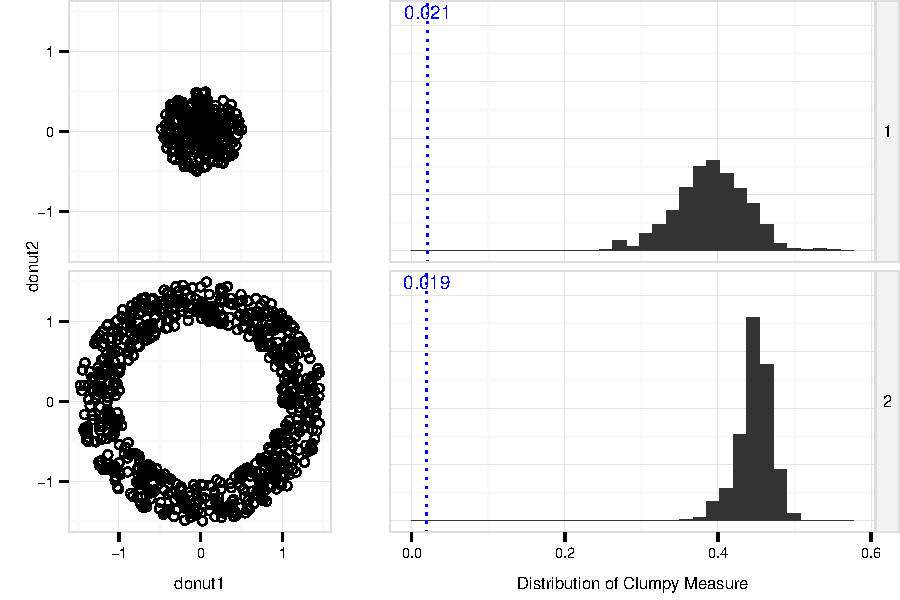
\includegraphics[width=1.5in]{images/19_7340782313668-cluster.pdf}
      \caption{}
      \label{fig:pars2}
      \end{subfigure}
      \begin{subfigure}[b]{\linewidth}
  	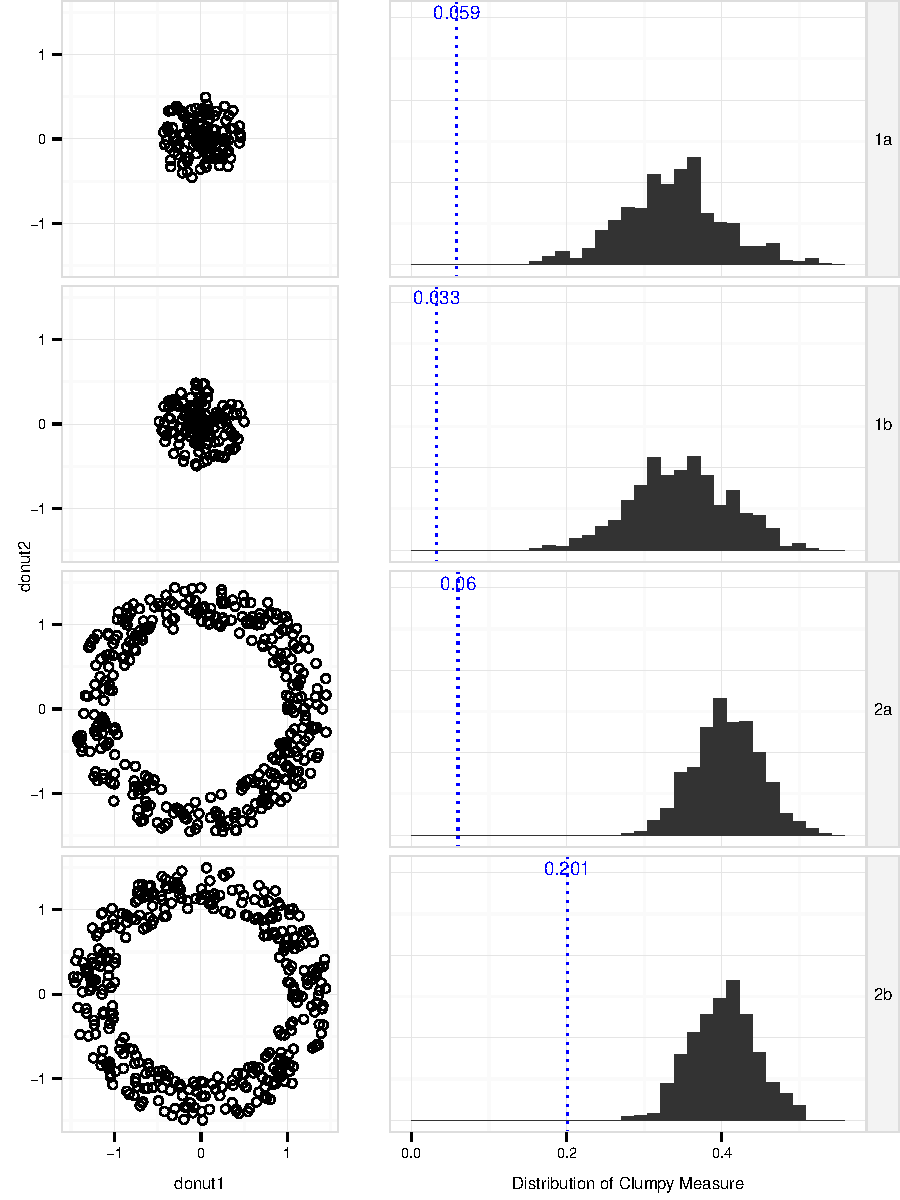
\includegraphics[width=1.5in]{images/8_12377386346542-cluster1.pdf}
        \caption{}
      \label{fig:pars3}        
      \end{subfigure}
    \end{minipage}
    \begin{subfigure}[b]{1.5in}
	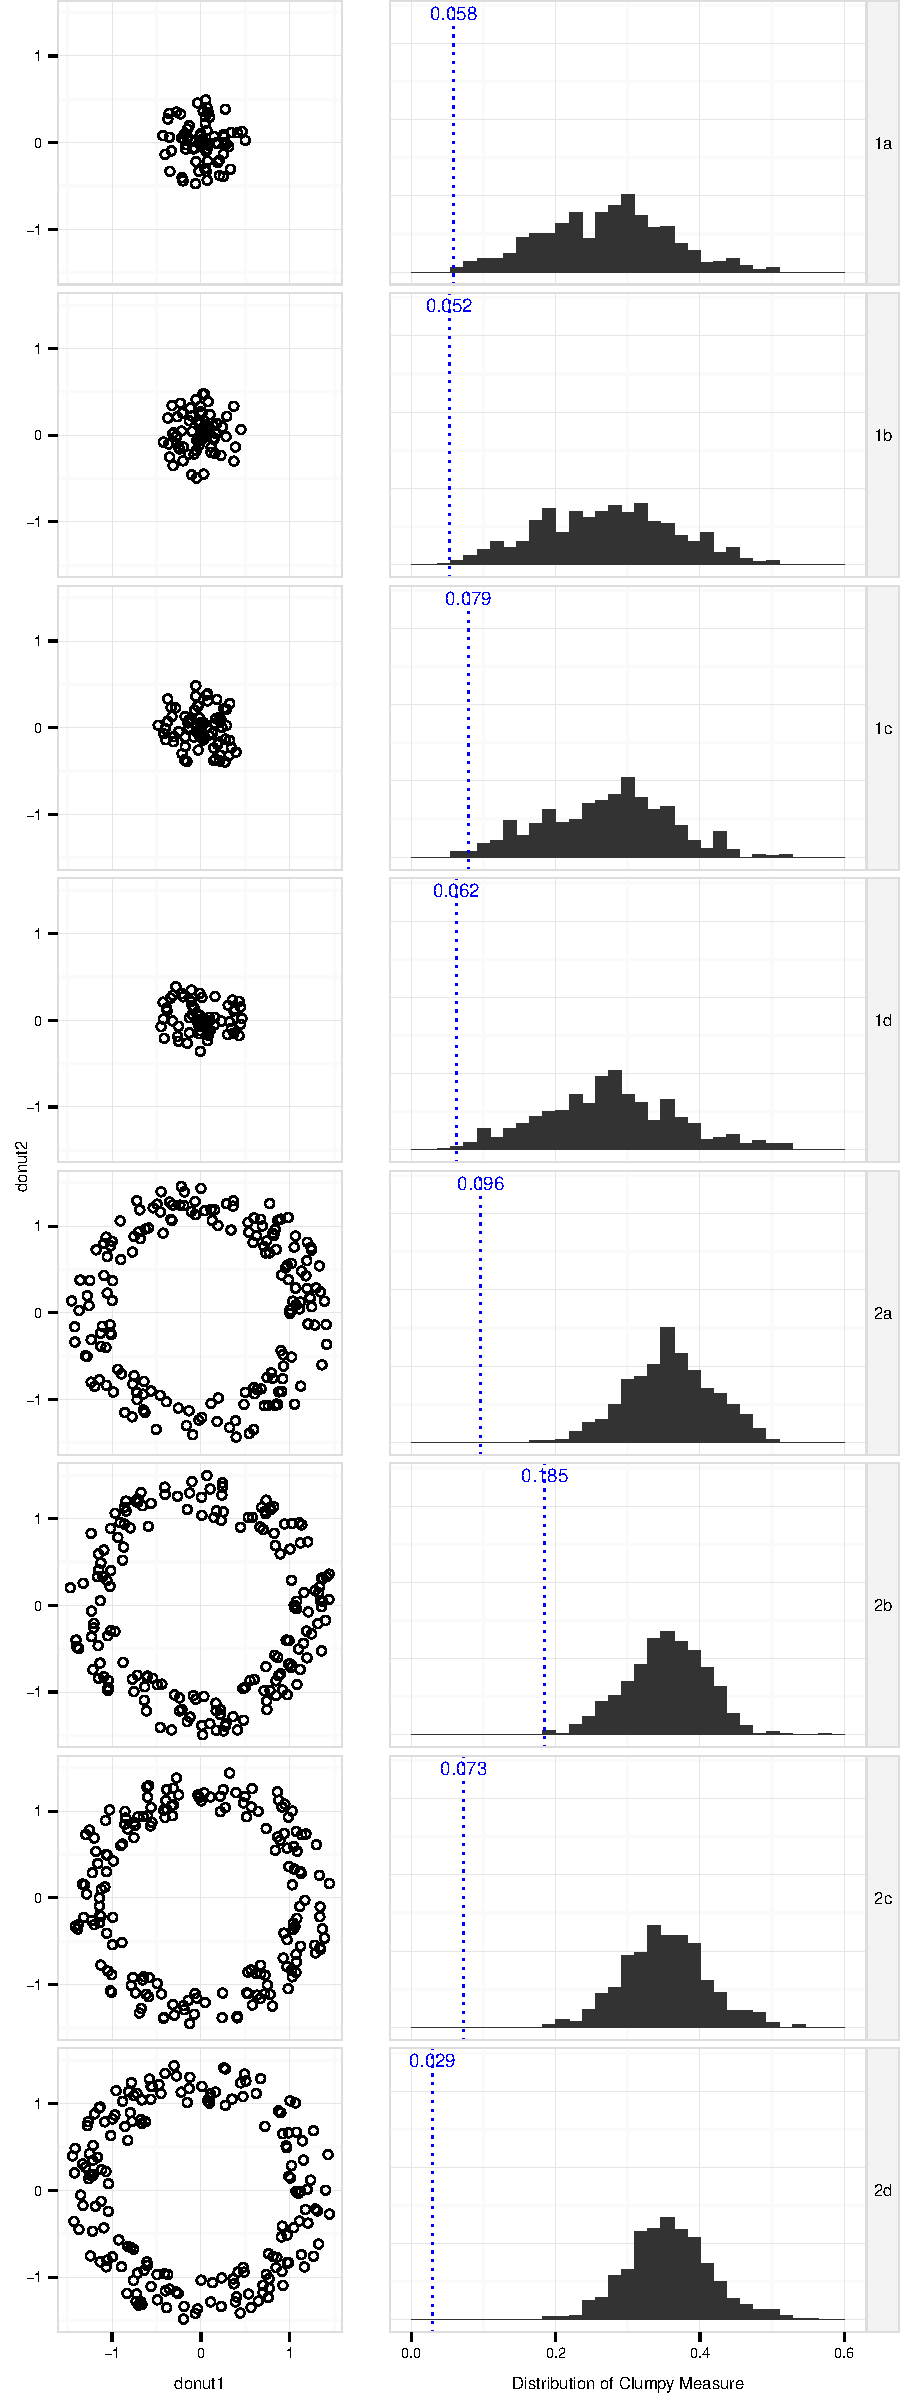
\includegraphics[width=1.5in]{images/5_54820204216055-cluster2.pdf}
      \caption{}
      \label{fig:pars4}
    \end{subfigure}
    \caption{The ranking of small multiple displays respects the parsimony criterion. (a) The original bullseye pattern. (b) The best small multiple determined by the Clumpy scagnostic. (c) The second best partitioning dimension redundantly halves the $2$ partitions from (b). (d) The lowest ranked small multiple display with $8$ partitions.}
    \label{fig:parsimonious}
  \end{figure}

High-cardinality Partitioners create a large number splits, which likely produce splits with low support as the observations get distributed among more facets. These small multiples are expectedly penalized by our approach as seen in Figure~\ref{fig:informative_sm_big}.

We examine the ability of our method to favor parsimonious small multiples using an artificially generated dataset so we can hold the visual patterns across partitioning dimensions equal as far as possible. We take the bullseye pattern shown in Figure~\ref{fig:pars1} and have a partitioning dimension that cleanly separates the ring from the core as seen in Figure~\ref{fig:pars2}. Then we create partitioning dimensions that repeatedly randomly halve the points in the partitions from the previous step to create small multiples as seen in Figures~\ref{fig:pars3} and~\ref{fig:pars4}. We compute the ranking of these partitioning dimensions and see the small multiples in the order as shown in Figure~\ref{fig:parsimonious}. We favor the parsimonious small multiple over the redundant ones that show similar visual patterns with low support. 

